\documentclass[
    %notes,
    aspectratio=169
]{beamer}
\usepackage[T2A]{fontenc}
\usepackage[utf8x]{inputenc}
\usepackage[english,russian]{babel}
\usepackage[T2A]{fontenc}
\usepackage[utf8x]{inputenc}
\usepackage[english,russian]{babel}
\usepackage{
  % cmap, % copy from pdf
  graphicx,
  subcaption,
  xcolor,
  caption,
  subcaption,
  hyperref, % for url in bibtex
  lineno,
  geometry,
  amssymb,
  amsfonts,
  amsmath, % for \begin{equation*}
  mathtext,
  cite,
  enumerate,
  float, % for figure with [ht]
  calc, % \widthof{999}
  amsthm
}
\newcommand{\bra}[1]{\left\langle #1 \right|}
\newcommand{\ket}[1]{\left| #1 \right\rangle}
\newcommand{\p}[1]{\left( #1 \right)}
\newcommand{\abs}[1]{\left| #1 \right|}
\newcommand{\tr}[1]{\mathrm{Tr} \left\{ #1 \right\}}
\newcommand{\sx}{I_\mathrm{x}}
\newcommand{\sy}{I_\mathrm{y}}
\newcommand{\sz}{I_\mathrm{z}}
\newcommand{\hdz}{H_\mathrm{dz}}
\graphicspath{{figures}}
\hypersetup{
  hidelinks, 
  unicode=true  % fix "PD1 encoding, removing `\CYRI'"
} 

% \setbeameroption{show notes on second screen}
\setbeamertemplate{caption}[numbered] % number figures
\usetheme{Madrid}
\title[Многочастичная запутанность]{Многочастичная запутанность}
\subtitle{в многоквантовой спектроскопии ЯМР в твердом теле}
\author[Лазарев И.Д.]{\textbf{И.Д. Лазарев\inst{1,2}}}
\institute[МГУ, ИПХФ РАН]
{
  \inst{1}%
  Московский государственный университет им. М. В. Ломоносова
  \and
  \inst{2}%
  Институт проблем химической физики РАН
}

\date[08.12.2022]{
Диссертация на соискание ученой степени кандидата физико-математических наук по специальности 1.3.8 - Физика конденсированного состояния \\
Научный руководитель д.ф.-м.н., профессор Э.Б. Фельдман 
}


\begin{document}

\frame{\titlepage}
\note{
    С прикладной точки зрения запутанность в квантовых системах является ресурсом для квантовых вычислений, коммуникации и других квантовых технологий. 
    Запутанность ответственна за преимущества квантовых приборов и устройств над их классическими аналогами. 
    % Изучение их свойств и методов управления ими является теоретической основой квантовых технологий.
    С фундаментальной точки зрения квантовая запутанность является ключевой концепцией квантовой механики, 
    и за частую играет важную роль во многих процессах. 
    Актуальной проблемой является развитие методов экспериментального исследования многочастичной запутанности. 
    В частности, оказалось, что в рамках МК спекстроскопии ЯМР можно существенно продвинуться в этом направлении. 

    Тема моей работы "Многочастичная запутанность в в многоквантовой спектроскопии ЯМР в твердом теле".
}

% \AtBeginSection[] {} % show display table of contest before new section
\begin{frame}
\frametitle{План доклада}
\tableofcontents
\end{frame}
\note{
  Во введении будет обсуждена проблематика и озвучена цель исследования.  
  
  Далее я познакомлю Вас с методами, которые позволяют исследовать многочастичную запутанность в рамках МК спектроскопии ЯМР. 

  Потом мы обсудим главные результаты. 
}

\section{Введение}
\begin{frame}{ЭПР-парадокс}
 \begin{columns}
   \column{0.4\textwidth}
   \begin{figure}
     \includegraphics[width=\textwidth]{bi-entanglement.png}
   \end{figure}

   \column{0.5\textwidth}
   \begin{block}{}
     Работа Эйнштейна—Подольского-Розена\footnote[frame]{A. Einstein, B. Podolsky, and N. Rosen \textit{Phys. Rev.} \textbf{47}, 777 (1935)}
     указывала на неполноту квантовой механики с помощью мысленного эксперимента,
     заключающегося в измерении параметров микрообъекта косвенным образом,
     без непосредственного воздействия на этот объект.
   \end{block}
   \begin{block}{}
      В 2008 году был проведен эксперимент\footnote[frame]{T. Scheidl et al. \textit{PNAS} \textbf{107}, 46, 19708-19713 (2010)},
      который подтвердил нелокальный\footnote[frame]{J.S. Bell \textit{Physics Physique Fizika} \textbf{1}, 195 (1964)}
      характер квантовой теории.
   \end{block}
 \end{columns}
\end{frame}
\note{
  В 35 году была опубликована ЭПР.
  Она указвывала на ...слайд...

  Джон Стюарт Белл предложил эксперимент который ...

  Первый эксперимент был проведен Джоном Клаузером в 1972 (википедия).
  Второй первый эксперимент был проведен Аленом Аспе в 70е.
  (Alain Aspect Phys. Rev. D 14, 1944 – Published 15 October 1976)
  И затем было еще много экспериментов.

  В 2010 году Джон Клаузер, Ален Аспе и Антон Цайлингер стали лауреатами премии Вольфа по физике «за фундаментальный концептуальный и экспериментальный вклад в основы квантовой физики, в частности за серию возрастающих по сложности проверок неравенств Белла (или расширенных версий этих неравенств) с использованием запутанных квантовых состояний»
}

\begin{frame}{Квантовые технологии}
  \begin{columns}
   \column{0.6\textwidth}
   \begin{figure}
     \begin{subfigure}[t]{0.33\textwidth}
       \includegraphics[width=\textwidth]{ultracold-atoms.png}
       %\captionsetup{labelformat=empty}
       \caption{Ultracold atoms}
       \label{fig:ultracold-atoms}
     \end{subfigure}
     \begin{subfigure}[t]{0.33\textwidth}
       \includegraphics[width=\textwidth]{ridberg-atoms.png}
       %\captionsetup{labelformat=empty}
       \caption{Rydberg atoms}
     \end{subfigure}
     % \vspace*{2mm}
     \vfill
     \begin{subfigure}[t]{0.33\textwidth}
       \includegraphics[width=\textwidth]{trapped-ions.png}
       %\captionsetup{labelformat=empty}
       \caption{Trapped ions}
     \end{subfigure}
     \begin{subfigure}[t]{0.33\textwidth}
       \includegraphics[width=\textwidth]{sycamore.png}
       %\captionsetup{labelformat=empty}
       \caption{SC qubits}
     \end{subfigure}
     \caption{
       Квантовые платформы.
       % (\ref{fig:ultracold-atoms})~{Bloch, I. Nature 453, 1016–1022 (2008)}
     }
   \end{figure}

   \column{0.4\textwidth}
   \begin{figure}
       \includegraphics[width=0.8\textwidth]{sycamore-supemancy.png}
       % \captionsetup{labelformat=empty}
       \caption{
         % F. Arute et al., Nature 574, 505 (2019)
         Nature 574, 505 (2019)
       }
     \end{figure}
   \end{columns}
\end{frame}
\note{
  Активная разработка квантовых компьютеров.
  Квантовые платформы и их сравнение.

  \textbf{ЯМР}
  ЯМР был первым, но он негодится для вычислений (нет чистых состояний).
  Отлично подходит для исследований.
  Много наработок.

  Исследуется все гильбертого пространство.
  Квантовое превосходство  на программируемом сверхпроводящем процессоре.
  Запутанные состояния являются важным ресурсом в квантовых вычисления:
  Например, недавно продемонстрированное группой Мартинеса квантовое превосходство [1] на программируемом сверхпроводящем процессоре связано с понятием запутанноси
}



\begin{frame}{Бинарная запутанность}
  \begin{columns}
    \column{0.57\textwidth}
    $$
      \left| \Psi \right\rangle
      = \frac{
        \left| \uparrow\uparrow \right\rangle +
        \left| \downarrow\downarrow \right\rangle
      }{\sqrt{2}}
    $$
    \begin{block}{Критерии запутанности}
      \begin{itemize}
        \item Энтропия фон-Неймана \\
          {\footnotesize C.H.Bennett et al. \textit{Phys. Rev. A} \textbf{54}, 3824 (1996)}
        \item Критерий Вуттеса \\
          {\footnotesize W.K. Wootters, \textit{Phys. Rev. Lett.} \textbf{80}, 2245 (1998)}
        \item Мера Шмидта \\
          {\footnotesize Eisert J. and Briegel H. J. \textit{Phys. Rev. A} \textbf{64}, 022306 (2001)}
        \item ...
      \end{itemize}
    \end{block}

    %\begin{example}
    %  Запутанность в нитрозильном комплексе железа (НКЖ)\footnote[frame]{S. M. Aldoshin, E. B. Feldman, and M. A. Yurishchev, \textit{JETP} \textbf{107}, 5, 804–811 (2008)}.
    %\end{example}

    \column{0.4\textwidth}
    %\vspace{-2mm}
    \begin{figure}
      \includegraphics[width=\textwidth]{bi-entanglement-jetp2008.png}
      \captionsetup{skip=-2mm}
      \caption{Температурная зависимость согласованности (1) и запутанности (2) для нитрозильного комплекса железа\footnote[frame]{S. M. Aldoshin, E. B. Feldman, and M. A. Yurishchev, \textit{JETP} \textbf{107}, 5, 804–811 (2008)}.}
    \end{figure}
  \end{columns}
\end{frame}
\note{
  На слайде приведен пример cостояния с бинарной запутанностью.
  Измерение одной частицы определяет состояние второй.

  Определения таких состояний не тривиальная задача.
  В действительности, чтобы показать, что состояние запутанно нужно еще угадать с проективными измерениями,
  так как в произвольном базисе нельзя установить факт наличия запутанности.

  Эта задача уже хорошо разработана
  и было предложено множество критериев для выявления таких корреляций.
  например  мера Шмидта, согласованность Вуттерса, энропия фон-Неймана.


  Этот эффект хорошо изучен экспериментально, в качестве примера
  на слайде приведен результат из работы нашего института.
  Это температурная зависимость величины запутанности
  подсчитаной на основе согласованности в нитрозильном комплексе железа.
  Линии это теоретический расчет, точки это эксперимент.

  Такие результаты удается получит благодаря тому, что согласованность
  Вуттерса связана с магнитной восприимчивостью атиферомагнитного димера.
}



\begin{frame}{Цели и задачи}
  \textbf{Целью данной работы} является теоретическое исследование многочастичной запутанности в системах с большим количеством частиц (>200) в рамках МК спектроскопии ЯМР,
а также развитие методов экспериментального измерения величин квантовой информации Фишера и косой информации Вигнера-Янасе.
\end{frame}


\section{Исследование квантовых корреляции методами ЯМР}

\subsection{Многочастичная запутанность}
\begin{frame}{Многочастичная запутанность}
  $$
  \left| \Psi_{3-\mathrm{ent}} \right\rangle
  = \frac{1}{\sqrt{8}}
  \left| \uparrow_1 \right\rangle
  \otimes
  \left(
    \left| \uparrow_2\uparrow_4\right\rangle +
    \left|\downarrow_2\downarrow_4\right\rangle
  \right)
  \otimes
  \left(
    \left|\uparrow_3\uparrow_5\uparrow_9\right\rangle +
    \left|\downarrow_3\downarrow_5\downarrow_9\right\rangle
  \right)
  \otimes
  \left(
    \left|\uparrow_6\uparrow_7\uparrow_8\right\rangle +
    \left|\downarrow_6\downarrow_7\downarrow_8\right\rangle
  \right)
  $$
  \begin{alertblock}{Многочастичная запутанность $k$-частиц}
  $$
  \left| \Psi_{k-\mathrm{ent}} \right\rangle
  	= \otimes^\mathrm{M}_{i=1} \left| \Psi_{i} \right\rangle,
  $$
  где $\left| \Psi_{i} \right\rangle$ это состояние подсистемы с $N_i$ частицами,
  $ \sum\limits_{i=1}^N N_i = N $
  и $ \exists m: N_{m} \ge k$
  \end{alertblock}

\end{frame}
\note{
  А вот многочастичная запутанность изучена гораздо хуже,
  так как для этого нужно исследовать многочастичные системы,
  пространство которой экспоненциально растет с увеличение числа частиц.

  Также не очевидно какое определение должнобыть у многочастичной запутанности.

  В нашей работе мы используем для многочастичной запутанности  следующее определение: ...слайд...

  То есть наличие запутанности порядка $k$,
  говорит о том что существует несепарабельная подсистема размера $k$.
}

\begin{frame}{Меры многочастичной запутанности}
  \vspace{-2mm}
  \begin{block}{Свойства}
    \begin{enumerate}
      \item $
        F(\rho_1 \otimes \rho_2 ,H_1 \otimes I_2 + I_1 \otimes H_2)
    	= F_{1} (\rho_1, H_1) + F_{2} (\rho_2 , H_2)
      $
      \item $F \leq N^2$
    \end{enumerate}
  \end{block}
  \vspace{-1mm}
  \begin{alertblock}{Уточнение верхней границы величины $F$}
    Пусть в системе максимальный размер несепарабельной подсистемы равен $k$, тогда
    $$ F^{k} \leq \left[ \frac N k \right] k^2 + \left(N - k \left[ \frac N k \right]\right)^2 $$
  \end{alertblock}
  \vspace{-1mm}
  \begin{examples}
    \begin{enumerate}
      \item Косая информация Вигнера-Янасе\footnote[frame]{Zeqian Chen \textit{Phys. Rev. A} \textbf{71}, 052302 (2005)}
      \item Квантовая информация Фишера\footnote[frame]{P. Hyllus et al. \textit{Phys. Rev. A} \textbf{85}, 022321 (2012)}
    \end{enumerate}
  \end{examples}
\end{frame}
\note{
 В настоящее время признано, что большинство физических процессов в природе можно сформулировать в терминах обработки информации, и концепция информации может быть центральной для понимания квантовой теории.


Нас интересует два свойства меры:
1. В сепарабельной системе с матрицей плотности $\rho = \rho_1 \otimes \rho_2$ квантовая информация Фишера удовлетворяет условию аддитивности)
2. Известна ее верхняя граница $F_\mathrm{Q} \leq N^2$, где $N$ это количество частиц в системе.

Благодаря этим свойствам, зная величину меры в системе можем оценить нижнюю границу количества запутанных частиц в системе. То есть если в системе максимальный размер не сепарабельной подистемы равен $k$, то
мера такой всей системы точно не больше данного значеничя: ...слайд...

Таким образом получив значение меры  выше при фиксированом $k$ ...слайд...,  мы можем утверждать что существует несепарабельная системы размера больше $k$ расчитать дать нижнюю оценку на минимальный размер несепарпбельной системы.

Какие величины имееют такие свойства?
В квантовой теории информации есть ...слайд...
Эти величины сами по себе очень интересные.
}


% \begin{frame}{Меры многочастичной запутанности}
% Фиксируем какое-то значение $k$ - максимальное количество спинов в несепарабельной подсистеме
% $$ N > k \geq N_1 \geq N_2 \geq \dots \geq N_l, \quad \sum_{i=0}^{l} N_i = N, $$
% где $l$ количество несепарабельных подсистем.
%
% Верхняя граница информации Фишера для такой системы:
% $$
% F^k = F_{1} + \dots + F_{l}
% \leq N^2_1 + \dots + N^2_e
% \leq \underbrace{
% 	k^2 + k^2 + \dots + k^2
% 	}_{m = \left[\frac N k \right] \, \mbox{раз}}
% 	+ \underbrace{(N-km)^2}_{\mbox{остаток}}
% $$
%
% \begin{alertblock}{}
%     $$  F^k \leq \left[ \frac N k \right] k^2 + \left(N - k \left[ \frac N k \right]\right)^2 $$
% \end{alertblock}
% \end{frame}
% \note{
% Доказательства этого факта сводится к вычислению верхней границы квантовой информации Фишера для с фиксированым размером не сепарабельных подсистем.
% Мы для себя фиксируем какое-то значение $k$ - максимальное количество спинов в несепарабельной подсистеме. Сделаем оценку сверху для информации Фишера.
%
% Пусть есть я ...
%
% Рассмотрим пару подсистем для которых верно $k > N_i > N_{i-1} > 0$.
% Квантовая информации Фишера этих двух подсистем:
% $$
% F_{Q\,i,i-1} \leq N_{i}^2 + N_{i-1}^2
% $$
% При этом если мы рассмотрим случай когда в правой системе на один спин меньше, а в левой на одим больше то оценка верхней границы будет выше:
% $$
% \bar F_{Q\,i,i-1}
% 	\leq \left( N_{i}^2 + 1 \right)
% 		+ \left( N_{i-1}^2 - 1\right)
% 	\leq N_{i}^2 + N_{i-1}^2
% 		+ 2 \left(N_{i} - N_{i-1} + 1 \right)
% $$
% Следовательно в худшем случае...???
%
% Следовательно если мы подсчитаем информацию Фишера, то мы
% можем дать нижнюю границу количества запутанных частиц.
% }

\subsection{Косая информация Вигнера-Янасе}
\section{Косая информация Вигнера-Янасе}
\label{sec:skew-wigner-yanase-information}
% история
% определение
% применение
% свойства
% формула
% связь c информацией Фишера
% связь со вторым моментом

% 10.1103/PhysRevLett.91.180403 Inro
% В исследовании измерения квантовомеханических операторов Вигнер показал, что наблюдаемые, которые не коммутируют с аддитивной сохраняющейся величиной, труднее измерить, чем те, которые коммутируют с сохраняющейся величиной; то есть, наличие закона сохранения накладывает ограничение на измерение наблюдаемых, которые несовместимы (не коммутируют) с сохраняющейся величиной [1,2]. Араки и Янасе строго установили, что наблюдаемые величины, не совпадающие с сохраняющейся величиной, не могут быть измерены точно (в смысле фон Неймана), возможно только приближенное измерение, и существует компромисс между "размером" измерительного прибора и точностью измерения [3,4]. Это составляет знаменитую теорему Вигнера-Араки-Янасе, которая накладывает принципиальное ограничение на измерение квантовомеханических наблюдаемых. Эта теорема в дальнейшем исследовалась многими авторами [5-9].
% Cледовательно наблюдаемые величины,
% которые коммутируют с аддитивными сохраняющимися величинами
% (энергия, компоненты линейного и углового моментов, электрический заряд),
% могут быть измерены с помощью микроскопических аппаратов,
% а те, которые не коммутируют с этими величинами, требуют для своего измерения макроскопических систем\cite{Wigner1960}.

%
%Согласно квантовомеханической теории,
% екоторые наблюдаемые величины могут быть измерены гораздо легче, чем другие:

Араки и Янасе строго установили, что наблюдаемые величины,
которые не являются интегралами движения,
не могут быть измерены точно (в смысле фон Неймана),
и возможно только приближенное измерение.
Согласно знаменитой теореме Вигнера-Араки-Янасе, которая накладывает принципиальное ограничение на измерение квантовомеханических наблюдаемых,
существует компромисс между ``размером'' измерительного прибора и точностью измерения\cite{Araki1961, Ozawa1991, Ozawa2002a, Ozawa2002b, Matsumoto1993, Kakazu3469}.
Наблюдаемые величины,
которые коммутируют с аддитивными сохраняющимися величинами
(энергия, компоненты линейного и углового моментов, электрический заряд),
могут быть измерены с помощью микроскопических аппаратов;
те же, которые не коммутируют с этими величинами, требуют для своего измерения макроскопических систем\cite{Wigner1960}.
Отсюда возникает проблема определения меры наших знаний относительно последних.

% Theoretical and Mathematical Physics, 202(1): 104–111 (2020)
Косая информация\cite{Wigner1963} была введена Вигнером и Янасе
в контексте квантовых измерений в качестве меры информации,
содержащейся в векторе квантового состояния, лежащего под углом по отношению к наблюдаемой $A$.
\begin{equation}\label{eq:wyi}
  I_{WY}(\rho, A)
  = -\frac{1}{2} Tr([\sqrt{\rho}, A])^2
  = Tr(\rho A^2) - Tr(\sqrt \rho A \sqrt \rho  A ).
\end{equation}
%
В частности, если $\rho = \ket{\psi}\bra{\psi}$ чистое состояние, тогда
%
\begin{equation}
  I_{WY}(| \psi \rangle, A)
  = \langle \psi | A^2 | \psi \rangle - \langle \psi | A| \psi \rangle ^2
\end{equation}

Косая информация Вигнера-Янасе существенно отличается от энтропии фон Неймана \cite{Wigner1960, Lieb1973prl, Lieb1973, Wehrl1978},
но глубоко связана с ней.
Энтропия, как ее обычно определяют, является мерой нашего незнания\cite{Weaver1949}.
Это мера, в которой знания о любой наблюдаемой величине находятся в одном ряду.
С точки зрения энтропии информационное содержание всех чистых состояний,
которые могут быть описаны одним вектором состояния, одинаково.
Это неверно для косой информации Вигнера-Янасе.
В отличие от вектора консервативной величины наблюдаемой $A$,
вектор состояния, лежащего наклонно к наблюдаемой $A$, содержит информацию.

Позднее было признано, что косая информация,
помимо своего изначального значения как меры информационного содержания состояний,
допускает также несколько интерпретаций,
носящих более физический и теоретико-информационный характер.
Например, Шунь Лун Ло показал\cite{Luo2003, Luo2005, Luo2005pra, Luo2006, Luo2017} ,
что косую информацию Вигнера-Янасе можно интерпретировать
как квантовую неопределенность наблюдаемой $A$ для квантового состояния $\rho$.

Интригующей и тонкой особенностью косой информации является использование в ней квадратного корня из оператора плотности квантового состояния.
Тем не менее популярность получили и естественные модификации косой информации Вигнера-Янасе,
в которых нет корня из оператора плотности.
Например, величина
%
\begin{equation}\label{eq:wyi-modification-l}
  L(\rho, A)
  = -\frac{1}{2} Tr([\rho, A])^2.
\end{equation}
%
Значительным преимуществом величины $L(\rho, A)$ в сравнении с косой информацией является возможность ее измерения экспериментально [12].
В [16] было показано,
что $L(\rho, A)$ можно измерить в "интерферометрической" установке (an interferometric setup) путем выполнения только двух программируемых измерений независимо от размерности квантовой системы.
Однако существует проблема зависимости $L(\rho, A)$ от характеристик вспомогательной системы, как было отмечено в [24].
С помощью сравнения косой информации с некоторыми ее естественными модификациями были раскрыты\cite{Luo2020} математические,
а также физические причины использования квадратного корня.

% Skew information has many nice properties and interpretations that make it useful in quantum information theory[1], [8].
В настоящее время косая информация Вигнера-Янасе нашла много применений в квантовой теории информации[1], [8].
% For example, skew information can be used to construct measures of quantum correlations [9]–[11],
% to quantify quantum coherence [12]–[15], to quantify asymmetry [15], and so on.
Например, информация о перекосе может быть использована для построения мер квантовых корреляций [9]-[11],
для количественной оценки квантовой когерентности [12]-[15],
для количественной оценки асимметрии [15] и так далее.
% It has also been used to study quantum phase transitions [16]–[20], uncertainty relations [6], [21]–[23], et cetera.
Она также использовалась для изучения квантовых фазовых переходов [16]-[20], соотношения неопределенностей [6], [21]-[23] и т.д.

Особенно нужно отметить,
что косая информация удовлетворяет свойствам из определения~(\ref{def:f}),
и, cледовательно, может быть использована для оценки количества запутанных частиц в системе.

% Chen2005


% ---- PRA
Тем не менее полноценное исследование многочастичной запутанность в системе
требует разработки соответствующих экспериментальных методов.
Основной недостаток квантовой информации Вигнера-Янасе заключается в том,
что эта величина не могла быть измерена экспериментально,
в отличии информации Фишера\cite{Garttner2018}.
Одним из главных достижений данной работы является преодоление этого препятствия.
В Главе~\ref{chapter:wyi-mesuarement} представлена теория экспериментального метода определения величины косой информации Вигнера-Янасе
в спиновой системе с диполь-дипольным взаимодействием в многоквантовом эксперименте ЯМР.
Оказывается,
что в этом случае косая информация Вигнера-Янасе тоже связана со значением
второго момента спектра интенсивностей многоквантовых когерентностей в системе.

% It is not a random magic because skew information may be identifier as a paradigmatic version of quantum Fisher information.
% % the statistical idea underlying the skew information is the Fisher information in the theory of statistical estimation.

\subsection{Квантовая информация Фишера}
\begin{frame}{Квантовая информация Фишера}
  \begin{block}{}
    Квантовая информация Фишера\footnote[frame]{D. Petz and C. I Ghinea, \textit{Quantum Probab. Relat. Top.} (2011)}
    показывает,
    как быстро изменяется квантовое состояние,
    определяемое матрицей плотности,
    при изменении некоторого параметра.
  \end{block}
  Квантовая информация Фишера --- это прямой аналог классической информации Фишера и основная мера в квантовой метрологии.
  Квантовая информация Фишера $F_Q$ для матрицы плотности $\rho$ по отношению к наблюдаемой $A$:
  $$
    F_Q \left(\rho, A \right) =
      2\sum_{j,k} \frac{\left(\lambda_j - \lambda_k \right)^2}
        {\lambda_j + \lambda_k}
      \left| \langle j|A|k \rangle \right|^2,
  $$
  где $\lambda_k$ и $|k \rangle$ --- собственное значение и собственный вектор матрицы плотности $\rho$.
\end{frame}
\note{
    Квантовая информация Фишера показывает, 
    как быстро изменяется квантовое состояние, 
    определяемое матрицей плотности, 
    при изменении некоторого параметра. 
    Как правило этот параметр является временем эволюции квантового состояния.

    Квантовая информация Фишера --- это прямой аналог классической информации Фишера, 
    и так как это скорость изменения состояния при изменении параметра часто используется в квантовой метрологии. 

    Далее мы сосредоточимся на квантовой информации Фишера. 
    так как для нее в МК эксперименте ЯМР возможно получить оценку снизу.
}


\subsection{Многоквантовая спектроскопия ЯМР}
\begin{frame}{Многоквантовый эксперимент ЯМР\footnote[frame]{
J. Baum, M. Munowitz, A. N. Garroway, and A. Pines, J. Chem. Phys. 83, 2015 (1985).}}

  \begin{figure}
    \includegraphics[width=0.5\textwidth]{mq-experiment-schema.pdf}
    %\caption{Схема МК эксперимента ЯМР}
  \end{figure}
  \vspace{-3mm}
  \begin{block}{}
    На подготовительном периоде МК эксперимента ЯМР система облучается последовательностью радиочастотных импульсов. В результате динамика спиновой системы определяется многоквантовым гамильтонианом.
    $$
    H_{MQ} = H^{(2)} + H^{(-2)},
    \quad H^{(\pm2)} = \frac 1 2 \sum_{i < j} D_{ij} I^\pm_i I^\pm_j
    $$
  \end{block}
\end{frame}
\note{
     МК динамику мы решили исследовать стандартным МК экспериментом.
     Эксперимент состоит из четырех частей,
     но нас будет интересовать только подготовительный период эксперимента.
     На подготовительном периоде ...слайд...
}

\begin{frame}{Многоквантовый экперимент ЯМР}
  \begin{columns}
    \column{0.4\textwidth}

    \begin{figure}
      \includegraphics[width=0.9\textwidth]{mq-experiment-pulses-schema.png}
      \caption{Схематичное представление последовательности импульсов МК эксперимента.}
    \end{figure}


    \column{0.6\textwidth}
    МК когерентности создаются в течение периода подготовки продолжительностью $\tau$ при участии m-серии 8-импульсовых подпоследовательностей и затем преобразуются в наблюдаемую намагниченность после идентичного периода смешивания (за исключением 90-градусного фазового сдвига). Затем намагниченность детектируется при импульсе $\pi/2$. Фазовый сдвиг $\phi$ между периодами подготовки и смешивания инкриминируется для разделения многоквантовых когерентностей разных порядков. В результате преобразования Фурье по $\phi$ получается МК ЯМР спектр.
    % Интенсивности МК когерентностей ЯМР при различных длительностях периода свободной эволюции $t$ получаются в отдельных экспериментах.
  \end{columns}
\end{frame}

\begin{frame}{Распределение интенсивности МК когерентностей ЯМР}
\begin{columns}
  \column{0.4\textwidth}
  \vspace{-3mm}
  \begin{figure}
    \includegraphics[width=\textwidth]{mq-coherence-intensities-hist.png}
    \caption{Распределение интенсивности МК когерентностей ЯМР.}
  \end{figure}

    \column{0.5\textwidth}
    \begin{block}{}
      Второй момент (дисперсия) распределения МК когерентностей ЯМР
      $$
        M_2 (\tau,\beta) = \sum_n n^2 J_n(\tau,\beta),
      $$
      где $J_n$ --- интенсивность МК когерентности ЯМР порядка $n$.
    \end{block}

\end{columns}
\end{frame}
\note{
  Подсчитать информацию фишера не просто подсчитить но она связана с рейльной физической величеной.
  Важно отметить что здесь нам удалось связать меру информации с физической величиной.
  Под действием гамильтониана происходят переходы между энергетическими уровнями
  и возникаюм многоквантовые когерентности.
  Гистограма показывает частоту этих переходов.
  ЯМР отличный инструмент и наша работа это подтверждает.

  % mq-coherences-distribution % JETP 2018
}



%\section{Измерение информации Фишера в МК эксперименте ЯМР}
%\begin{frame}{Определение информации Фишера в МК ЯМР (PRA-19)\footnote{S.I. Doronin, E.B. Fel'dman,  I.D. Lazarev, \textit{Phys. Rev. A}, \textbf{100}, 022330 (2019)}}
  $$ G(\tau, \phi) =
     \mathrm{Tr}\left\{
         e^{iH_\mathrm{MQ}\tau} e^{i\phi I_z} e^{-iH_\mathrm{MQ}\tau}
         \rho_\mathrm{eq}
         e^{iH_\mathrm{MQ}\tau} e^{-i\phi I_z} e^{-iH_\mathrm{MQ}\tau}
         I_z \right\}
  $$
  \begin{alertblock}{}
      Дисперсия распределения интенсивности МК когерентностей ЯМР определяет нижнюю границу информации
      Фишера\footnote[frame]{
      M. G\"arttner, P. Hauke, and A.M. Rey. \textit{Phys. Rev. Lett.} \textbf{120}, 040402 (2018)}:
      $$
      F_Q \geq 2M_2
      $$
  \end{alertblock}
  Однако формула справедлива только в том случае,
  если сигнал $G(\tau, \varphi)$ является \textit{out-of-time-ordered correlator} (OTOC).
  Для низких температур это условие не выполняется.
  Возможно обойти это ограничение,
  если усреднить сигнал МК эксперимента ЯМР по начальному состоянию:
  $$ G_\mathrm{LT}(\tau, \phi)
     = \mathrm{Tr}\left\{
       e^{iH_\mathrm{MQ}\tau} e^{i\phi I_z} e^{-iH_\mathrm{MQ}\tau}
       \rho_\mathrm{eq}
       e^{iH_\mathrm{MQ}\tau} e^{-i\phi I_z} e^{-iH_\mathrm{MQ}\tau}
       {\color{red} \rho_\mathrm{eq}}
    \right\}
  $$
\end{frame}




\section{Многочастичная запутанность в системе эквивалентных спинов}
\begin{frame}{Система эквивалентных спинов}
  \begin{figure}
    \begin{subfigure}[t]{0.32\textwidth}
      \includegraphics[width=\textwidth]{model-nanopore-schema.png}
      \caption{
        Hанопора\footnote[frame]{J. Baugh, A. Kleinhammes, D. Han, Q. Wang, and Y. Wu, \textit{Science} \textbf{294}, 1505 (2001).},
        заполненная спин-несущими молекулами во внешнем сильном магнитном поле $\vec B$.
      }
    \end{subfigure}
    \hfill
    \begin{subfigure}[t]{0.32\textwidth}
      \includegraphics[width=0.8\textwidth]{sample-nanopore-nmr-spectrum.png}
      \caption{
        Молекулярная диффузия газа быстрее флип-флоп процессов.
        Вся система характеризуется одной константой $D$.
      }
    \end{subfigure}
    \hfill
    \begin{subfigure}[t]{0.32\textwidth}
      \includegraphics[width=\textwidth]{sample-nanopore-film.png}
      \caption{
        Значение константы связи $D$ зависит как от газа,
        так и от эффективного давления в нанопоре ($\approx 1$ кБар)
      }
    \end{subfigure}
    \captionsetup{skip=-0.1mm}
    \caption{}
  \end{figure}

  % \begin{block}{Нанопора\footnote[frame]{J. Baugh, A. Kleinhammes, D. Han, Q. Wang, and Y. Wu, Science 294, 1505 (2001).}, заполненая частицами со спином $1/2$}
  %     Так как молекулярная диффузия газа быстрее флип-флоп процессов,
  %     вся система характеризуется одной константой взаимодейсвия $D$.
%
  %     \vspace{\baselineskip}
%
  %     Значение константы связи $D$ зависит как от газа, так и от эффективного давления в нанопоре ($\approx 1$ кБар).
  % \end{block}
\end{frame}
\note{
    Hydrogenated amorphous silicon (Гидрогенизированный аморфный кремний)

    Для исследования многочастичной запутанности нам нужна модель,
    в которой почти все частицы взаимодействуют друг с другом,
    а также она должна поддаваться счету.
    Мы решили рассмотреть модель эквивалентных спинов.
    Такой модели соотвествует нанопора заполеннея спин несущими частицами.

    Такие нанопоры получаются выдавлием под давлением ~ 1 кБар  на специальной подложке.

    Необходимо подчеркнуть, что существуют некоторые ограничения для реализации описанной модели при исследовании нанопористых соединений с МК - ЯМР-методами. Например, модель предполагает, что все нанопоры имеют одинаковый объем и одинаковую "несферическую" форму.

    Молекулярная диффузия газа очень быстрая в сравнениидиподьных флип флом процессов
    Каждая частица успевает обойти всю нанопору пока пройдет флипфлоп
    Поэтому можно описать взаимодействие с одной константой

    Среднняя константа связи зависит как от газа, так и от эффективного давления в нанопоре

    При низких температурах диффузия побеждает?
    Какие частицы?
}

\begin{frame}{Диагонализация гамильтониана}
Многоквантовый гамильтониан
$$
H_\mathrm{MQ} = - \dfrac{D}{4} \left\{
    \left( I^{+} \right)^2 + \left( I^{-} \right)^2
\right\}
$$
коммутирует с проектором квадрата полного углового момента
$ \left[ H_\mathrm{MQ}, \hat I^2 \right] = 0 $.
Следовательно, в базисе собственных значений  $\hat I^2$ и $I_z$  гамильтониан имеет блочно-диагональный вид :
$$
H_\mathrm{MQ} = \mathrm{diag} \left\{
    H_\mathrm{MQ}^{N/2},
    H_\mathrm{MQ}^{N/2 - 1},
    \dots
    H_\mathrm{MQ}^{N/2 - [N/2]}
\right\},
$$
где каждый блок соответствует собственному значению полного углового момента.
\end{frame}
\note{
    Так как в нашей модели все констаны одинаковые, МК гамильтониан упрощается.
    Этот гамильтониан коммутирует ...слайд...
}

\begin{frame}{Эволюция информации Фишера (PRA-19)}
  \begin{figure}
    \begin{subfigure}[t]{0.3\textwidth}
      \includegraphics[width=\textwidth]{m2_t_b01.pdf}
      \caption{$\beta = 0.1$}
    \end{subfigure}
    \begin{subfigure}[t]{0.3\textwidth}
      \includegraphics[width=\textwidth]{m2_t_b05.pdf}
      \caption{$\beta = 0.5$}
    \end{subfigure}
    \begin{subfigure}[t]{0.3\textwidth}
      \includegraphics[width=\textwidth]{m2_t_b3_5.pdf}
      \caption{$\beta = 3.5$}
    \end{subfigure}
    \caption{Зависимость нижней границы информации Фишера от времени.}
  \end{figure}
\end{frame}


\begin{frame}{Температурная зависимость многочастичной запутанности (PRA-19)}
\begin{columns}
    \column{0.5\textwidth}
    \begin{figure}
    \includegraphics[width=0.7\textwidth]{k_b.pdf}
    \caption{Зависимость числа запутанных частиц от обратной температуры.}
    \end{figure}


    \column{0.5\textwidth}
    В начальный момент времени система находится в термодинамическом равновесии:
    $$
    \rho_\mathrm{eq} = \dfrac{ e^{\beta I_z} }{Tr \left\{ e^{\beta I_z} \right\} },
    \quad
    \beta = \dfrac{\hbar \omega_0}{k_{B} T}
    $$
\end{columns}
\end{frame}
\note{
При понижении температуры количество запутанных частиц стремительно растет.

При достаточно низкой температуре почти все спины запутаны друг с другом,
даже когда начальное состояние не было запутанно.

}


\begin{frame}{Дипольное упорядочение (JETP-20)\footnote{I.D. Lazarev and E.B. Fel'dman , \textit{JETP} \textbf{131}, 5, (2020)}}
  \alert{При дипольно упорядоченном начальном состоянии когерентности возникают быстрее:}
  $$
  \rho_i = \frac{1}{Z_i} e^\frac{\hslash\beta_\mathrm{d} \hdz}{k}
  \approx \frac{1}{Z_i}(1 + \frac{\hslash\beta_\mathrm{d}}{k} H_\mathrm{dz}),
  $$
  то есть зеемановская температура низкая, а дипольная --- высокая.
  \begin{block}{Методы создания дипольно упорядоченного состояния}
    \begin{itemize}
      \item  Адиабатическое размагничивание\footnote[frame]{C. P. Slichter and W. C. Holton, Phys. Rev. 122, 1701 (1961)} от большого значения приложенного поля до нуля во вращающейся системе координат.

      \item Двухимпульсный эксперимент Броекаерта-Джинира\footnote[frame]{J. Jeener and P. Broekaert, Phys. Rev. 157, 232 (1967).}.
  \end{itemize}
  \end{block}
\end{frame}
\note{

Был рассмотрен случай низкой зеемановской и высокой дипольной температурами, когда начальное состояние является

%Поэтому представляется целесообразным попытаться непосредственно охладить ядерную спиновую систему, используя то обстоятельство, что она относительно изолировапа от решетки из-за слабости механизмов спин-решеточной релаксации.

%Наиболее прямой метод охлаждения ядерных моментов заключается в их адиабатическом размагничивании от большого значепия приложенного поля до пуля. При обычных условиях охлаждение, получаемое этим способом, оказывается недостаточным.

%Например, адиабатическое размагничивание ядерной спиновой системы, выполняемое, скажем, при температуре решетки $Т_0 = 1$К, начиная с поля $H0 = 25 кЭ$, приводит к конечной температуре $T_f ~ T_0 H_L / H_0$, где величина локального поля $H_L$ состав­ляет несколько эрстед. В этом случае конечная темпера­тура будет порядка $10^{-4}$ К, что по крайней мере на два порядка превосходит требуемое зпачение.

Эксперимент Броекаерта-Джинира удобнее так как это естественные

Однако подходы, разработанные для этих исследований, ограничены случаем высоких температур и не могут применяться для изучения многоспиновой запутанности.

Но нам удалось теоретически доказать что двухимпульсная последовательность Брокаерта – Джинера [17, 19] позволяет получить дипольное упорядоченное состояние даже при низкой зеемановской температуре.

Также важно отметить, что гамильтониан Hdz частично усредняется быстрой молекулярной диффу- зией в нанопоре, а усредненный гамильтониан мож- но записать как
}

% \begin{frame}{Получение дипольно упорядоченого состояния}
% В начальный момент времени система находится в термодинамическом равновесии
% %
% $$
%     \rho(0) = \rho_\mathrm{eq} = \frac{1}{Z}
%     e^{
%       \frac{\hslash \omega_{0}}{k} \alpha_\mathrm{z} I_\mathrm{z}
%       + \frac{\hslash }{k} \beta_\mathrm{d} H_\mathrm{dz}
%     }
% $$
% %
% где $Z$ --- статистическая сумма; \\
% $\alpha_\mathrm{z}$, $\beta_\mathrm{d}$ --- обратные зеемановская и дипольная температуры; \\
% $H_\mathrm{dz}$ --- секулярная часть гамильтониана ДДВ в сильном внешнем магнитном поле;
% $$
%     H_\mathrm{dz} = \frac{D}{2} (3 I^{2}_{z} - I^{2})
% $$
% Нас интересует случай,
% когда зеемановская температура низкая, а дипольная --- высокая
% $$
%     \frac{\hslash \omega_{0}}{k} \alpha_\mathrm{z}\gg 1,
%     \quad\quad
%     \frac{\hslash D}{k}\beta_\mathrm{d} \ll 1
% $$
% \end{frame}
% \note{
%     В начальный момент времени ...
%     И мы уже рассмотрели этот случай в 19 году.
%     Однако в случае дипольного упорядочения когерентности...
%     А как я говорил, дисперсия распределеяня когерентностей связана с количеством запутанных частиц.
% }


\begin{frame}{Эволюция информации Фишера (JETP-20)}
  \begin{figure}
    \begin{subfigure}[t]{0.3\textwidth}
    \includegraphics[width=\textwidth]{eval-1.png}
    \caption{$T = 6 \times 10^{-4}$ K}
    \end{subfigure}
    \hfill
    \begin{subfigure}[t]{0.3\textwidth}
      \includegraphics[width=\textwidth]{eval-2.png}
      \caption{$T = 3.2 \times 10^{-4}$ K}
    \end{subfigure}
    \hfill
    \begin{subfigure}[t]{0.3\textwidth}
      \includegraphics[width=\textwidth]{eval-3.png}
      \caption{$T = 4.8 \times 10^{-5}$ K}
    \end{subfigure}
    \caption{Зависимости нижней границы квантовой информации Фишера $F_Q = 2M_2$ от безразмерного времени $D\tau$ при $N = 101$.}
  \end{figure}
\end{frame}
\note{
    Нам удалось решить динамику для этой системы и изучить систему при разных значения температуры и размера системы.
}

\begin{frame}{Дипольное упорядочение (JETP-20)}
    \begin{figure}
    \includegraphics[width=0.7\textwidth]{entangled_spins_by_n.eps}
    \caption{
      Зависимости минимального количества числа запутанных частиц,
      усредненного по времени эволюции, от температуры.
     }
    \end{figure}
\end{frame}
\note{
мы хотели поймать скачак количества запутанных состояний, поэтому рассмотрели упорядочение

Максимальное количество запутанных спинов при одинаковой температуре увеличивается, когда увеличивается число спинов в нанопоре, потому что система в нанопоре становится плотнее.
}


\section{Многочастичная запутанность в квазиодномерных цепочках}
\begin{frame}{Однородная цепочка спинов}
  \begin{columns}
    \column{0.35\textwidth}
    \begin{figure}
      \includegraphics[width=\textwidth]{sample-fap-crystal-structure-part.png}
      \caption{Фтористый апатит Ca$_{10}$(PO$_4$)$_6$F$_2$}
    \end{figure}

    \column{0.6\textwidth}
      Часть кристаллической структуры FAp, показывающая окружение атомов фтора.
      Атомы кислорода были удалены для ясности.
      Атомы фтора равномерно разнесены ($r_{FF}= 3.44$\AA) и расположены в колонны вдоль $c$-оси кристалла.
      Каждый атом фтора окружен тремя равноудаленными атомами фосфора при $r_{FP} = 3.67$\AA,
      которые расположены в вершинах равносторонних треугольников на плоскости, перпендикулярной к $c$-оси,
      а также тремя ионами Ca\textrm{II} на расстоянии $2.34$\AA.
  \end{columns}
\end{frame}
\note{
  Фтористый апатит.
}

\begin{frame}{Альтернированная цепочка}
\begin{columns}

    \column{0.3\textwidth}
    \begin{figure}
    \includegraphics[width=1.0\textwidth]{model-zigzag-chain-schema.png}
    \caption{}
    \end{figure}

    \column{0.6\textwidth}
    \begin{block}{Константы взаимодействия}
        $$D_1=\dfrac{\gamma^2\hbar }{r^3}, $$
        $$D_2 = D_1\dfrac{ 3\cos^2 \varphi -1 }{2} $$
        $$D_3 = D_1 \dfrac{ 3\sin^2 \frac{\varphi}{2} -1}{16 \sin^3, \frac{\varphi}{2}}$$
        где $\gamma$ - гиромагнитное отношение,
        $\varphi$ - угол между соседними связями,
        $r$ - расстояние между соседними спинами в цепочке.
    \end{block}

\end{columns}
\end{frame}
\note{
    Базовый случай это когда одна линия связи направлена вдоль поля. тогда констаты будет самой большой в доль поля.
    Изменяя угол к полю мы можем получить как альтернированную цепочку так и однородную.
    В приближении ближайших и следующих соседей, задача решается аналитически, но она
    не дает полной картины. Поэтому мы решали данную систему численно.
}

\begin{frame}{Альтернированная цепочка (JMR-20)\footnote[frame]{
        G.A. Bochkin and et al., \textit{J. Magn. Res.} \textbf{319}, 106816, (2020)}}
\begin{columns}

    \column{0.4\textwidth}
    \begin{figure}
      \includegraphics[width=0.85\textwidth]{model-zigzag-chain-hambergite-structure.png}
      \caption{}
    %\caption{Hанопора со спин-несущих молекулами во внешнем сильном магнитном поле $\vec B$}
    \end{figure}

    \column{0.6\textwidth}
    \begin{block}{Гамбергит $Be_2BO_3(OH)$ }
        \begin{itemize}
            \item Дипольное взаимодействия между ближайшими спинами протонов в цепи в 17 раз сильнее, чем со спинами окружающих цепей (в худшем случае).
            \item Взаимодействия с остальными окружающими спинами по меньшей мере в 30 раз слабее.
            \item Вклад дипольной связи между спинами в одной и той же цепи доминирует над остальными взаимодействиями.
        \end{itemize}
    \end{block}

\end{columns}
\end{frame}
\note{
    В одномерных цепочках возникают когерентности только $\pm 2$ порядка
    и следовательно дисперсия распределения будет небольшой
    и мы не увидим запутанных кластеров.
    Однако в альтернированная цепочке гамбергита возникают когерентности $\pm 4$ порядка
    и следовательно можно использовать эту модель для исследования многочастичной запутанности.
    The distance to these two protons is 4.49 Å
    The distance between a given chain and surrounding proton chains is at least 2.1 times larger than the distance between neighbors in the chain.

  % JMR 2020
}
\begin{frame}{Эволюция нижней границы информации Фишера}
% (AMR-20)\footnote{G.A. Bochkin et al., \textit{Appl. Magn. Res.} \textbf{51}, 667-678, (2020)}
\begin{columns}

    \column{0.6\textwidth}
    \begin{figure}
    
\includegraphics[width=0.95\textwidth]{result-zchain-m2-by-time-n6-beta10.eps}
    %\caption{Hанопора со спин-несущих молекулами во внешнем сильном магнитном поле $\vec B$}
    \end{figure}

    \column{0.4\textwidth}
    Зависимость нижней границы квантовой информации Фишера
    $$ F_Q = 2M_2(\tau, T) $$
    от безразмерного времени $D_1 \tau$
    для шести спинов
    при температуре $T = 2.5 \times 10^{-3}$ $(\beta = 10)$.
    Область многочастичной запутанности ограничена горизонтальными линиями $k = 1$, $k = 5$.
\end{columns}
\end{frame}
\note{
   Мы не можем точно сказать сколько спинов запутанно,
   но можем дать нижнюю оценку на количество запутанных между собой спинов.
}


\begin{frame}{Максимальное количество запутанных спинов}
\begin{columns}

    \column{0.5\textwidth}
    \begin{figure}
    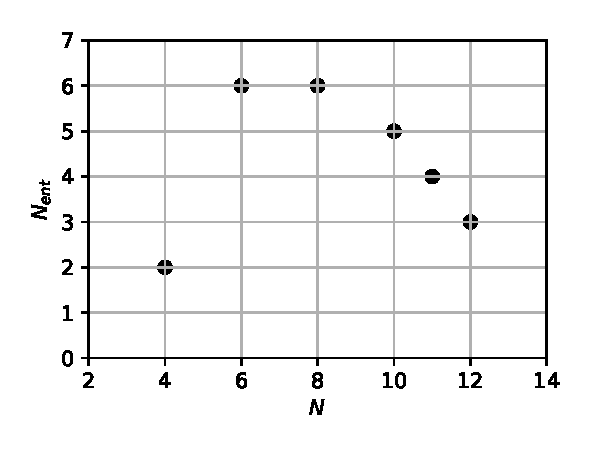
\includegraphics[width=\textwidth]{result-zchain-nent-by-n-beta10.eps}
    \caption{}
    \end{figure}

    \column{0.5\textwidth}
    Зависимость максимального количества запутанных спинов $N_\mathrm{ent}$ от длины цепи при температуре $T = 2.5 \times 10^{-3}$ $(\beta = 10)$.

    \vspace{0.5cm}

    \alert{Создание запутанных кластеров в рассматриваемых зигзагообразных цепочках ограничено слабыми дипольными взаимодействиями удаленных спинов}.
\end{columns}
\end{frame}
\note{
  Установлено что, при фиксированной температуре с ростом числа спинов в цепи размер запутанных кластеров может уменьшаться;
}


\begin{frame}{Максимальное количество запутанных спинов}
  \begin{columns}
     \column{0.5\textwidth}
     \begin{figure}
     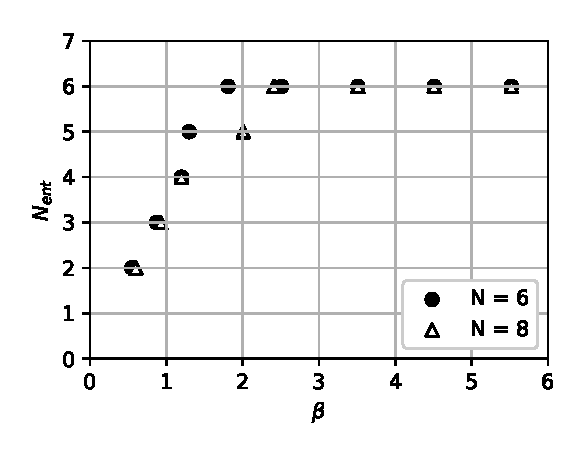
\includegraphics[width=\textwidth]{result-zchain-nent-by-beta-n8-n6.eps}
     \caption{}
     \end{figure}

     \column{0.45\textwidth}
     \begin{block}{}
       Зависимость максимального количества запутанных спинов $N_\mathrm{ent}$ от обратной температуры
       $$ \beta = \dfrac{\hbar\omega_0}{kT} $$
       в зигзагообразной цепочки из 6 и 8 спинов.
    \end{block}
  \end{columns}
\end{frame}
\note{
    Для 6 спинов накачка происходит быстрее, чем для 8 спинов.
}


\section{Измерение информации Вигнера-Янасе в МК эксперименте ЯМР}
\chapter{Измерение информации Вигнера-Янасе в МК эксперименте ЯМР}
\label{chapter:wyi-mesuarement}

% PLA-2021

% \section{Многоквантовая динамика при низких температурах}
% \input{slides/results/mq-dynamic-at-low-temperature}
%
% \section{Многоспиновая запутанность в системе эквивалентных спинов}
% \input{slides/models/equivalent-spins}
% \input{slides/results/equivalent-spins-entanglement-with-term-equilibrium-state}
% \input{slides/results/equivalent-spins-entanglement-with-dipolar-ordered-state}
%
% \section{Многоспиновая запутанность в цепочках}
% \input{slides/models/zigzag-spin-chain}
% \input{slides/results/zigzag-spin-chain-entanglement}
%
% \section{Определение информации Вигнера-Янасе в МК эксперименте ЯМР}
% \input{slides/results/determination-of-wigner-yanase-information}
%
% \section{Сравнение информации Вигнера-Янасе и Фишера}
% \input{slides/results/comparison-wyi-and-fi}

\section{Итоги}
\begin{frame}{Положения, выносимые на защиту}
  \begin{enumerate}
  \item
  Разработанная теория МК ЯМР позволяет исследовать многочастичную запутанность в системе ядерных спинов при произвольной температуре.

  \item
  С понижением температуры количество запутанных спинов растет и в нанопоре, и в зигзагобразной цепочке. 
  % В нанопоре, заполненой спин несущими частицами, при температуре 
  % $T = 6.856\cdot10^{-3}$~K $(\beta=3.5)$ 
  % почти все спины (до 179 из 201) запутаны.
  %Исследована температурная зависимость многочастичной запутанности в нанопоре,
  %когда система приготовлена в термодинамическом равновесном зеемановском и дипольном упорядоченном состояниях.

  \item
  Оценка количества запутанных спинов в однородных цепочках согласуется с результатами, представленными в литературе.
  % Исследована многочастичная запутанность в квазиодномерных цепочках ядерных спинов в зависимости от параметров цепи и температуры.

  \item
  Если спиновая система исследуется в МК эксперименте ЯМР с начальным равновесным термодинамическим состоянием при температуре $T$, 
  то ее косая информация Вигнера-Янасе равна удвоенному второму моменту распределения интенсивностей МК когерентностей ЯМР системы, приготовленной при вдвое большей температуре $2T$ в тот же момент времени эволюции;
  % Предложен метод экспериментального измерения точного значения косой информации Вигнера-Янасе в рамках МК спектроскопии ЯМР.

  \item
  Результаты оценки количества запутанных спинов, полученные на основе квантовой информации Фишера и косой информации Вигнера-Янасе, согласуются;
  % Проведено сравнение оценок многочастичной запутанности, 
  % полученных на основе квантовой информации Фишера и косой информации Вигнера-Янасе.
\end{enumerate}

\end{frame}

\begin{frame}{Публикации}
  \begin{thebibliography}{}
    \documentclass[a4paper, 14pt]{extreport}
\usepackage[T2A]{fontenc}
\usepackage[utf8x]{inputenc}
\usepackage[english,russian]{babel}
\usepackage{
  % cmap, % copy from pdf
  graphicx,
  subcaption,
  xcolor,
  caption,
  subcaption,
  hyperref, % for url in bibtex
  lineno,
  geometry,
  amssymb,
  amsfonts,
  amsmath, % for \begin{equation*}
  mathtext,
  cite,
  enumerate,
  float, % for figure with [ht]
  calc, % \widthof{999}
  amsthm
}
\begin{document}
\section*{Публикации по теме диссертации}
\begin{enumerate}
  \bibitem{Doronin2019} S. I. Doronin, E. B. Fel'dman,  I. D. Lazarev, Many-particle entanglement in multiple quantum nuclear-magnetic-resonance spectroscopy, \textit{Physical Review A}, \textbf{100}, 022330 (2019)
\bibitem{Lazarev2020} I. D. Lazarev and E. B. Fel'dman, Many-Spin Entanglement in Multiple Quantum NMR with a Dipolar Ordered Initial State,  \textit{JETP}, \textbf{131}, 5, (2020)
\bibitem{Bochkin2020a} G.A. Bochkin, E.B. Fel'dman, E.I. Kuznetsova, I.D. Lazarev, S.G. Vasil'ev, V.I. Volkov, 1H NMR in a quasi-one-dimensional zig-zag spin chain of hambergite, Be2BO3(OH), \textit{Journal of Magnetic Resonance}, \textbf{319}, 106816, (2020)
\bibitem{Bochkin2020b} G. A. Bochkin, S. I. Doronin, E. I. Kuznetsova, I. D. Lazarev, E. B. Fel’dman, S. G. Vasil’Ev, Many‐Spin Entanglement in Zigzag Spin Chain in Multiple Quantum NMR, \textit{Applied Magnetic Resonance}, \textbf{51}, 667-678, (2020);
\bibitem{Doronin2021} S. I. Doronin, E. B. Fel'dman,  I. D. Lazarev, Multiple quantum NMR in solids as a method of determination of Wigner–Yanase skew information, \textit{Physics Letters A}, \textbf{406}, 127458 (2021)
\end{enumerate}
\thispagestyle{empty} % omit page number
\end{document}
  \end{thebibliography}
\end{frame}

\begin{frame}{Благодарности}
  И.Д. Лазарев выражает благодарность научному руководителю профессору Э.Б. Фельдману
и коллегам
Г.А. Бочкину,
С.Г. Васильеву,
С.И. Доронину,
А.И. Зенчуку,
Е.И. Кузнецовой,
и А.H. Пыркову.

И.Д. Лазарев выражает признательность за поддержку Фонду развития теоретической физики и математики ``Базис'' (№19-1-5-130-1).

Работа выполнена при поддержке фонда Министерства Науки и Высшего Образования Российской Федерации (№075-15- 2020-779) и частично (№075-15-2020-788).
\end{frame}

% \input{slides/suplemental-materials}

\begin{frame}{Ацаркин Вадим Александрович}
\begin{enumerate}
    \item В качестве критического замечания отмечу, что в диссертации, на мой взгляд, недостаточно подробно обсуждены конкретные преимущества использования именно многочастичной запутанности в квантовых вычислениях. Какие реальные перспективы открывает такой подход, имеются ли уже достоверные оценки – или же это дело отдаленного будущего? 

    \item Сходная проблема возникает и с низкими температурами. В ряде случаев теоретически изученные диссертантом температурные диапазоны (милликельвины) пока малодоступны. Понятно, что эти исследования устремлены в будущее, это похвально и необходимо. Тем не менее, хотелось бы более четко представлять себе перспективу. 
\end{enumerate}

\end{frame}

\begin{frame}{Погосов Вальтер Валентинович}
\begin{enumerate}
    \item При рассмотрении многоспиновой запутанности в квазиодномерных цепочках в главе 4 используется гауссово приближение для распределения интенсивностей многоквантовых когерентностей. Остается неясным, насколько оправдано это приближение и как выход за его рамки может поменять результат.

    \item В главе 5 на рис. 5.1 приведены зависимости оценки снизу числа запутанных спинов от обратной температуры на основе квантовой информации Фишера и на основе косой информации Вигнера-Янасе. Несмотря на качественное согласие между этими результатами имеются существенные количественные отличия. С чем они связаны, и которая из оценок более адекватна? 

    \item В диссертации практически отсутствует качественное рассмотрение. 
\end{enumerate}
\end{frame}

\begin{frame}{Цуканов Александр Викторович}
\begin{enumerate}
    \item Автор классифицирует запутанность многочастичных систем по количеству запутанных частиц. Возможна ли дальнейшая классификация запутанности при уже зафиксированном числе запутанных частиц? Например, для описания парной запутанности существует параметр согласованности, который варьируется от 0 до 1 и позволяет не только установить факт запутывания двух частиц, но и степень их запутанности (0 – частицы не запутаны, 1 – частицы запутаны максимально). 

    \item Рассмотрена фермионная система частиц с полуцелым спином. Адаптируется ли данная схема для бозонов – фотонов или атомных частиц с целым спином? 
\end{enumerate}

\end{frame}

\end{document}
